%
\documentclass[10pt]{article}

% The usual packages
\usepackage{fullpage}
\usepackage{breakcites}
\usepackage{setspace}
\usepackage{endnotes}
\usepackage{float}
\usepackage{amsmath}
\usepackage{amsfonts}
\usepackage{amssymb}
\usepackage{rotating}
\usepackage{dcolumn}
\usepackage{longtable}
\usepackage{microtype}
\usepackage{graphicx}
\usepackage{hyperref}
%\usepackage[usenames,dvipsnames]{color}
\usepackage{url}
\usepackage{natbib}
\usepackage{framed}
\usepackage{epigraph}
\usepackage{lipsum}
\usepackage{subcaption}
\usepackage{parskip}
\usepackage{hanging}
\usepackage[left]{lineno}

\usepackage[font=small,labelfont=sc]{caption}
%\restylefloat{table}
\bibpunct{(}{)}{;}{a}{}{,}

% place figures at the end
\usepackage{endfloat}
\renewcommand{\listoffigures}{} % but suppress these lists
\renewcommand{\listoftables}{} % suppress these lists

% Set paragraph spacing the way I like
\parskip=0pt
\parindent=20pt

% Define mathematical results
\newtheorem{lemma}{Lemma}
\newtheorem{proposition}{Proposition}
\newtheorem{theorem}{Theorem}
\newtheorem{claim}{Claim}
\newenvironment{proof}[1][Proof]{\begin{trivlist}
\item[\hskip \labelsep {\bfseries #1}]}{\end{trivlist}}
\newenvironment{definition}[1][Definition]{\begin{trivlist}
\item[\hskip \labelsep {\bfseries #1}]}{\end{trivlist}}
\newenvironment{example}[1][Example]{\begin{trivlist}
\item[\hskip \labelsep {\bfseries #1}]}{\end{trivlist}}
\newenvironment{remark}[1][Remark]{\begin{trivlist}
\item[\hskip \labelsep {\bfseries #1}]}{\end{trivlist}}

% Set up fonts the way I like
%\usepackage{tgpagella}
%\usepackage[T1]{fontenc}
%\usepackage[bitstream-charter]{mathdesign}

%% Set up lists the way I like
% Redefine the first level
\renewcommand{\theenumi}{\arabic{enumi}.}
\renewcommand{\labelenumi}{\theenumi}
% Redefine the second level
\renewcommand{\theenumii}{\alph{enumii}.}
\renewcommand{\labelenumii}{\theenumii}
% Redefine the third level
\renewcommand{\theenumiii}{\roman{enumiii}.}
\renewcommand{\labelenumiii}{\theenumiii}
% Redefine the fourth level
\renewcommand{\theenumiv}{\Alph{enumiv}.}
\renewcommand{\labelenumiv}{\theenumiv}
% Eliminate spacing around lists
\usepackage{enumitem}
\setlist{nolistsep}

% Create footnote command so that my name
% has an asterisk rather than a one.
\long\def\symbolfootnote[#1]#2{\begingroup%
\def\thefootnote{\fnsymbol{footnote}}\footnote[#1]{#2}\endgroup}

% Create the colors I want
\usepackage{color}
\definecolor{darkred}{RGB}{100,0,0}

\hypersetup{
pdftitle={Unreliable Inferences about Unobserved Processes}, % title
pdfauthor={Carlisle Rainey and Robert A. Jackson}, % author
pdfkeywords={partial observability} {split population}
pdfnewwindow=true, % links in new window
colorlinks=true, % false: boxed links; true: colored links
linkcolor=black, % color of internal links
citecolor=black, % color of links to bibliography
filecolor=black, % color of file links
urlcolor=blue % color of external links
}

% enable comments in pdf
\newcommand{\kelly}[1]{\textcolor{darkred}{#1}}
\newcommand{\carlisle}[1]{\textcolor{magenta}{#1}}

% April 6 Statistics Politics Policy submission
\begin{document}
%\linenumbers
\begin{center}
{\LARGE \textbf{Unreliable Inferences about Unobserved Processes}\\\vspace{2mm}
{\large \textbf{A Critique of Partial Observability Models}}\symbolfootnote[1]{We thank Will Moore, Austin Mitchell, participants at the 2012 Southern Political Science Association Annual Conference, and participants at the 2012 Midwest Political Science Association Annual Conference for valuable comments on previous versions of the manuscript. All code and data necessary to replicate the simulations and empirical analysis are available at \url{http://github.com/carlislerainey/unreliable-inferences}.}}

\vspace{10mm}

Carlisle Rainey\symbolfootnote[2]{Carlisle Rainey is Assistant Professor of Political Science, Texas A\&M University, 2010 Allen Building, College Station, TX, 77843 (\href{mailto:crainey@tamu.edu}{crainey@tamu.edu}).}

\vspace{3mm}

Robert A. Jackson\symbolfootnote[3]{Robert A. Jackson is Professor of Political Science, Florida State University, 531 Bellamy Building, Florida State University, Tallahassee, FL 32306 (\href{mailto:rjackson@fsu.edu}{rjackson@fsu.edu}).}
\end{center}

\vspace{10mm}

% Abstract
{\centerline{\textbf{Abstract}}}
\begin{quote}\noindent
Methodologists and econometricians advocate the partial observability model as a tool that enables researchers to estimate the distinct effects of a single explanatory variable on two partially observable outcome variables. 
However, we show that when the explanatory variable of interest influences both partially observable outcomes, the partial observability model estimates are unusually sensitive to misspecification. 
We use Monte Carlo simulations to show that minor, unavoidable misspecification of the functional form can lead to large bias under partial observability, even though such misspecification leads to little or no bias under full observability.
 \end{quote}
\vspace{10mm}
% Add quote to first page
\epigraph{The data may not contain the answer. The combination of some data and an 
aching desire for an answer does not ensure that a reasonable answer can be extracted from a given body of data.}{John Tukey (1986, p. 74)}

\vspace{10mm}
\begin{center}
Word Count: 4,426
\end{center}

% Remove page number from first page
\thispagestyle{empty}

% Start main text
\newpage
\doublespace

\section*{Introduction}

Social scientists often face situations, known as ``partial observability,'' where two (or perhaps more) distinct processes lead to distinct binary outcomes that can only be observed jointly. 
Braumoeller (2003) provides many examples of established literature theorizing such relationships. 
Econometricians and methodologists argue that researchers can use a partial observability model to parse out the effects of a single explanatory variable on each unobserved outcome (Poirier 1980; Abowd and Farber 1982; Pzeworski and Vreeland 2002; Xiang 2007; Nieman 2015).  

Partial observability models inform the literatures on important processes and outcomes such as civil wars (Nieman 2015), international conflict and trade (Xiang 2010), IMF agreements (Knight and Santaella 1997, Przeworski and Vreeland 2000, 2002, Vreeland 2003, and Stone 2008), union membership (Abowd and Farber 1982), regulatory compliance (Feinstein 1990, Stafford 2002, Chen et al. 2006, and Wang 2013), network formation (Comola and Fafchamps 2014), credit ratings (Boyes, Hoffman, and Low 1989), agricultural innovation (Dimara and Skuras 2003), health insurance ownership (Amir 2001), and employment discrimination (Heywood and Mohanty 1990, Logan 1996, and Mohanty 2002). 
Feinstein (1990) suggests the model's usefulness for a wide range of policy studies, and the model appears to hold out promise for investigating numerous other subjects, including deterrence, treaty compliance, and attitudes and behaviors that are subject to social desirability bias when measured via a survey report (Beger et al. 2011). 

In spite of the optimistic application of the partial observability model, we argue that researchers should view these estimates with some suspicion. 
We show that seemingly innocuous and unavoidable specification errors that lead to little or no large-sample bias under full observability can lead to a substantial large-sample bias under partial observability.

\section*{A Partial Observability Logit Model}

Partial observability occurs when the researcher can only observe a binary outcome of interest $d_{main}$ jointly with another binary outcome $d_{nuisance}$.\footnote{For clarity, we imagine a situation where one outcome is of interest and the other is largely nuisance. 
However, our ideas generalize to a situation where the researcher's interest extends to both outcomes.}
The researcher can directly observe the binary outcome $y$, which equals one if both $d_{main}$ and $d_{nuisance}$ equal one and zero otherwise.\footnote{One can also employ a partial observability model where $y$ equals one if either $d_{main}$ of $d_{nuisance}$ equals one. 
For simplicity, we focus on a situation where $y$ equals one if both $d_{main}$ and $d_{nuisance}$ equal one. 
Our conclusions do not depend on this choice.}

To model the observed outcome $y$, we assume that $d_{main}$ and $d_{nuisance}$ are independent events so that $\Pr(y) = \Pr(d_{main})\Pr(d_{nuisance})$.\footnote{Especially in the case of the partial observability probit model, the researcher can relax the assumption of independence. 
We make the assumption of independence to simplify the presentation and the computation.} 
Next, we assume a standard model relating a set of covariates $X = [1, w_1, w_2,..., w_{k_w}, x_1, x_2,..., x_{k_x}]$ to $\Pr(d_{main})$ and a set of covariates $Z = [1, w_1, w_2,..., w_{k_w}, z_1, z_2,..., z_{k_z}]$ to $\Pr(d_{nuisance})$, so that $\Pr(d_{main}) = g^{-1}(X\beta)$ and $\Pr(d_{nuisance}) = g^{-1}(Z\gamma)$.
Note that the covariates $w_j$ for $j \in \{1, 2,..., k_w\}$ belong to both $X$ and $Z$. 
This is crucial---our critique focuses on the situation where the researcher wishes to parse out the distinct effects of one or more explanatory variables on \textit{both} unobservable outcome variables.\footnote{Even if the researcher \textit{assumes} that each explanatory variable influences only one of the observable outcomes, we usually have only weak theory guiding the choice and no empirical tools to verify the assumption.} 
The researcher's theory rarely offers a compelling rationale for a particular link function $g$, making the choice essentially arbitrary (King 1998, p. 100, and Berry, DeMeritt, and Esarey 2010).
In our partial observability model, we let $g$ be the logit function, but other standard choices include probit, cloglog, and cauchit.
Using this form, it is straightforward to find the log-likelihood function for $\beta$ and $\gamma$, although the maximization is not trivial.\footnote{We find that standard hill-climbing optimization routines find local maxima. 
This presents a separate, perhaps equally concerning problem to substantive applications. 
To avoid this, we tried an algorithm suggested by Sekhon and Mebane (1998) that relies on a combination of genetic adaptation and hill-climbing to efficiently locate the maximum (Mebane and Sekhon 2011). 
This approach consistently located the global maximum in several trial examples, but only for a very large population (i.e., computationally prohibitive) of agents. 
We found that starting a standard hill-climbing algorithm at several sets of random starting values consistently located the global maximum. 
We use ten sets of starting values in our estimation.} 
We assume that the researcher uses the estimates of $\beta$ and $\gamma$ to calculate some quantity of interest (e.g., first difference). 
As a comparison, we also consider a full observability logit model (i.e., the usual logit model), where the researcher observes $d_{main}$ and uses the model $\Pr(d_{main}) = \text{logit}^{-1}(X\beta)$ to estimate the quantity of interest.

\section*{A Motivating Example}

To illustrate the potential bias with a simple example, suppose the researcher wants to estimate $\beta$ and $\gamma$ in the stylized model
\begin{gather*}
\Pr(d_{main}) = \text{logit}^{-1}(\beta x)\nonumber\\
\Pr(d_{nuisance}) = \text{logit}^{-1}(\gamma x - z)\nonumber\\
\Pr(y) = \Pr(d_{main})\Pr(d_{nuisance})\text{,}\nonumber
\end{gather*}
where $y$ represents the binary outcome of interest, $x$ and $z$ represent two binary explanatory variables, and $\beta$ and $\gamma$ represent parameters to be estimated. 
Suppose further that $(\beta, \gamma) = (-1, 1)$ or $(\beta, \gamma) = (1, -1)$ so that the researcher knows the absolute value of $\beta$ and $\gamma$ is 1, but is not sure which parameter is negative.

Because $x$ and $z$ are binary, there are four conditions, and we can easily compute the expected proportions under each for both sets of possible parameters. 
Table \ref{tab:ep} shows these proportions, where $\delta$ represents the logit$^{-1}$ function for compactness. 
The only difference in the expected proportion occurs when $x = 1$ and $z = 1$, where $(\beta, \gamma) = (-1, 1)$ produce an expected proportion of 0.13 and $(\beta, \gamma) = (1, -1)$ produce an expected proportion of 0.09.

\begin{table}[h]
    \begin{subtable}{.5\linewidth}
      \centering
        \caption{}
\begin{tabular}{crr}
\multicolumn{3}{c}{$(\beta, \gamma) = (-1, 1)$}\\ \hline
 & \multicolumn{1}{c}{$z = 0$} & \multicolumn{1}{c}{$z = 1$}\\
$x = 0$ & $\delta(0)\delta(0) = 0.25$ & $\delta(0)\delta(-1) = 0.13$\\
$x = 1$ & $\delta(-1)\delta(1) = 0.20$ & $\delta(-1)\delta(0) = \textbf{0.13}$\\\hline
\end{tabular}
    \end{subtable}%
    \begin{subtable}{.5\linewidth}
      \centering
        \caption{}
\begin{tabular}{ccc}
\multicolumn{3}{c}{$(\beta, \gamma) = (1, -1)$}\\ \hline
 & \multicolumn{1}{c}{$z = 0$} & \multicolumn{1}{c}{$z = 1$}\\
$x = 0$ & $\delta(0)\delta(0) = 0.25$ & $\delta(0)\delta(-1) = 0.13$\\
$x = 1$ & $\delta(1)\delta(-1) = 0.20$ & $\delta(1)\delta(-2) = \textbf{0.09}$\\\hline
\end{tabular}
    \end{subtable} 
        \caption{Expected proportional under the two possible parameter combinations of the stylized partial observability model.}\label{tab:ep}
\end{table}

This raises the question: How much would we need to alter the logit link function so that we obtain Panel A of Table \ref{tab:ep} with parameters $(\beta, \gamma) = \{1, -1\}$? The answer is ``not much.''

Our goal is to replace the function logit$^{-1}$ with a new function $h^{-1}$ to obtain Panel A of Table \ref{tab:ep} with parameters $(\beta, \gamma) = (1, -1)$. 
The only time we use $\text{logit}^{-1} (-2)$ in the calculation is for the bottom-right cell. In that case, let $h^{-1}(x) = \text{logit}^{-1}(x)$ for $x \in c\{ -1, 0, 1\}$. 
This ensures that all but the bottom-right cell remains unchanged. 
Then we require that 
\begin{align*}
h^{-1}(-2)h^{-1}(1) &= 0.13\\
h^{-1}(-2)\text{logit}^{-1}(1) &= 0.13\\
h^{-1}(-2) &= \frac{0.13}{\text{logit}^{-1}(1)}\\
h^{-1}(-2) &= \frac{0.13}{0.73}\\
h^{-1}(-2) & = 0.18 \text{ (as opposed to logit$^{-1}(-2) = 0.12$)}
\end{align*}
Figure \ref{fig:example} compares the functions logit$^{-1}$ and $h^{-1}$, which are similar, yet lead to exactly \textit{opposite} inferences about the effects of $x$ on $d_{main}$ and $d_{nuisance}$. 
If the researcher obtains a large set of data with proportions identical to Panel A of Table \ref{tab:ep}, then her conclusion about the effects of $x$ on $d_{main}$ and $d_{nuisance}$ depends on her assumption about the link function. 
If she assumes the logit link function, then she concludes that $x$ has a large, \textit{negative} effect on $d_{main}$. 
If she assumes the link function $h$, then she concludes that $x$ has a large, \textit{positive} effect on $d_{main}$. 
This example clearly highlights how minor errors in model specification can lead to large bias. 
To show the potential for bias in a broader collection of situations, we now turn to two simulation studies.

\begin{figure}[h]
\begin{center}
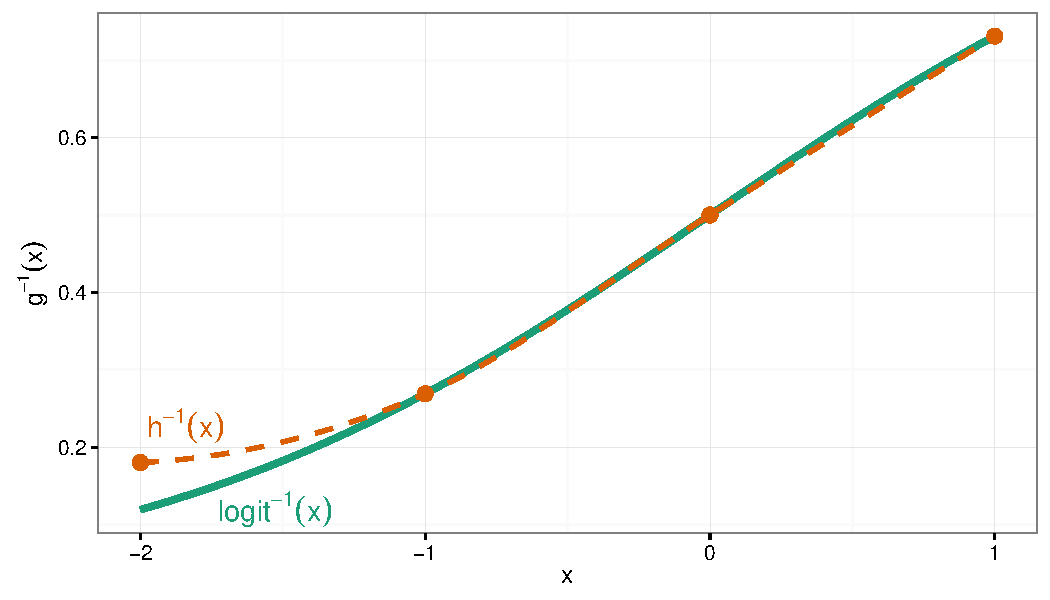
\includegraphics[scale = .6]{figs/example.pdf}
\caption{This figure compares the link functions logit$^{-1}$ and $h^{-1}$ that lead to exactly opposite inferences in the stylized partial observability model.}\label{fig:example}
\end{center}
\end{figure}

\section*{Simulation Studies}

We use two simulation studies to support our claim that partial observability models are highly sensitive to seemingly innocuous specification errors. 
In the first study, we evaluate the bias in the partial observability logit model estimates as the link function $g$ of the true data-generating process (DGP) varies. 
We view this as a highly conservative test of our claim, but find that misspecifying the link function can lead to large biases. 
In the second study, we consider more severe misspecifications of the functional form. 
Berry, DeMeritt, and Esarey (2015) observe that few social science theories offer more precision than a simple monotonic relationship between an explanatory variable and the probability of an event. 
Motivated by their observation, we evaluate the performance of the partial observability logit model for a variety of monotonic DGPs.
The simulations clearly show that (1) neither type of misspecification introduces much bias into the estimate under full observability and (2) both types of misspecification can introduce large bias into the estimate under partial observability, including sign errors.

\subsection*{Simulation Study 1: Wrong Link Function}

Many researchers view the choice of link function in a model of a binary outcome as an arbitrary, unimportant choice. 
Berry, DeMeritt, and Esarey (2015) summarize this idea:
\begin{quote}
In the typical study using binary logit or probit, the theory introduced is not sufficiently specific to imply that logit, probit, or any other functional form is a good fit to the hypothesized DGP. 
Instead, logit or probit is chosen from among the countless possible functional forms for a model simply because logit and probit have come to be viewed as ``default'' estimators for a binary dependent variable model---making them convenient estimation choices.\footnote{The authors continue in a footnote:
\begin{quote}
For example, the 2005 issues of three major journals---American Journal of Political Science (AJPS), American Political Science Review (APSR), and The Journal of Politics (JOP)---contain 49 articles studying binary dependent variables with logit or probit; 30 of these articles offer no defense for their choice of logit or probit; ten other papers defend their choice, but solely by noting that the dependent variable is dichotomous. 
\end{quote}}
\end{quote}
We endorse and echo the authors' key point: in the social sciences, researchers rarely have a strong theoretical justification for choosing one functional form over another. 

Given that researchers seldom have a compelling reason to prefer a logit model over a probit model, a cloglog model, or a cauchit model, we would find it especially troubling if the ability of the partial observability model to recover the quantity of interest depends on the researcher choosing the proper link function. 
Our simulations show exactly this---if the researcher chooses the wrong link function (e.g., uses a partial observability \textit{logit} model for a \textit{cauchit} DGP), then the large-sample estimates can have substantial bias.

To assess the large-sample bias of the partial observability model we simulate 500 large data sets for each of our DGPs (i.e., 100 million observations for each unique combination of the values for each explanatory variable). 
Across each data set, we randomly vary $k_w$, $k_x$, $k_z$, $\beta$, and $\gamma$. 
We also randomly vary the type of each explanatory variable, either binary or continuous. 
For each random set of simulation parameters, we simulate a large data set using logit, probit, cloglog, and cauchit DGPs.  
For each data set, we use the partial observability logit model to estimate the first difference as the key variable of interest $w_1$ varies from its minimum to its maximum. 
To ensure comparable first differences, we rescale $\beta$ and $\gamma$ appropriately for each link function. Section \ref{app:mon} of the Appendix summarizes the details of the algorithm.

Figure \ref{fig:link} shows the large-sample estimates of the first difference. 
The left-hand column shows the relationship between the estimated and true effect under full observability, where misspecifying the link function has almost no effect on the inferences. 
The largest biases under full observability occur for the cauchit DGP, where the average absolute bias is less than 0.01. 
The average absolute true effect is about 0.1, so the average absolute bias is relatively small. 
Most importantly, though, the estimate almost always falls close to the true value regardless of the DGP. 
For the worst-case cauchit DGP, the 95th percentile of the absolute bias is about 0.04 and the maximum is 0.08. 
The correlations between the estimated effect and the true effect for a cauchit DGP is 0.99.
These minor biases are expected; the cauchit link function is nearly indistinguishable from the logit link function and there is almost never a compelling theoretical reason to prefer one over the other. 

\begin{figure}[h]
\begin{center}
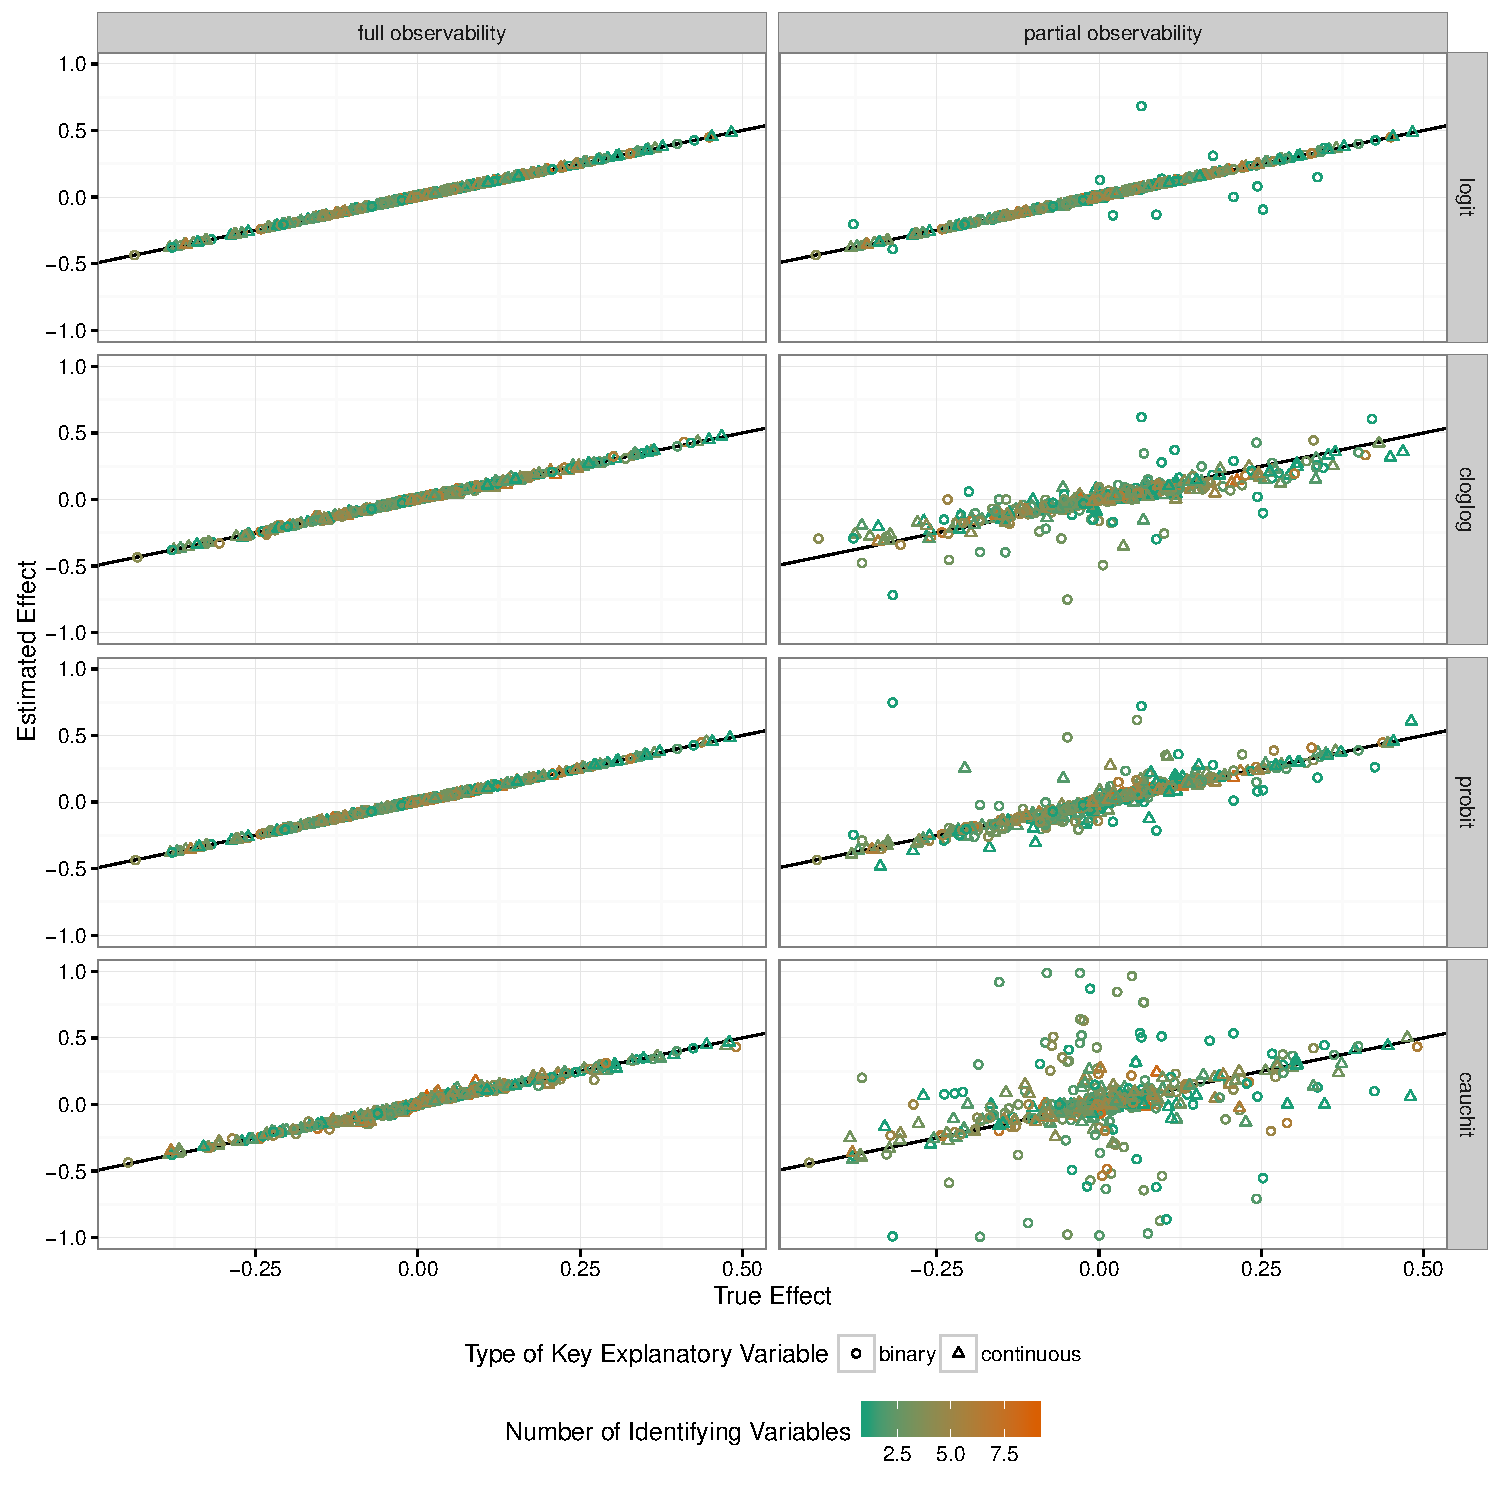
\includegraphics[scale = .6]{figs/link-sims-scatter.pdf}
\caption{These scatterplots show the large-sample estimates of the first difference as the true first difference varies. The left column shows the estimates under full observability (i.e., usual logit model) and the right column shows the estimates under partial observability. The top row shows the estimates when the link function is specified correctly as logit. The remaining rows show the estimates when the link function is not specified correctly (i.e., specified as logit when the DGP is probit, cloglog, and cauchit).}\label{fig:link}
\end{center}
\end{figure}

The results under partial observability, though, tell a different story---the bias can be much larger. 
For the cauchit DGP, the average absolute bias is about 0.07 when $w_1$ is continuous and about 0.20 when $w_1$ is binary---about 7 and 20 times larger under partial observability than under full observability, respectively. 
Under partial observability, the correlation between the estimated effect and the true effects drops to 0.69 when $w_1$ is continuous and to 0.32 when $w_1$ is binary.
And remember that standard errors do not reflect this large-sample bias and that the bias does not shrink as the sample size increases. 
This performance differential does not occur because the partial observability model requires more information to estimate the parameters; it occurs because the partial observability model is highly sensitive to misspecification. 

Unlike the full observability model, the partial observability model does not guarantee an estimate close to the true value. 
For the cauchit DGP, the 95th percentile for the average absolute bias is about 0.17 and the maximum is about 0.30 when $w_1$ is continuous. When $w_1$ is binary, the 95th percentile is 0.83 and the maximum is 1.12. 
Though the researcher has made only a small specification error, this small error produces a moderate-to-large bias on average and an enormous bias on occasion. 
Perhaps most informatively, for the cauchit DGP, the partial observability logit model produces sign errors in 24\% of the simulations when $w_1$ is continuous and in 31\% of the simulations when $w_1$ is binary. 
That is, when using a partial observability logit model to estimate a cauchit DGP, not only does the estimate converge to the wrong value (i.e., is inconsistent), it often converges to a value with the wrong sign!
In contrast, the full observability logit model does not produce a single sign error in our simulations, regardless of the DGP.

While the cauchit DGP acts as the worst-case scenario for the partial observability logit model, the biases that emerge for the probit DGP are especially telling. 
The conventional wisdom suggests that the choice between a logit and probit model is inconsequential. 
Indeed, King (1998, p. 100) notes in passing that the two link functions ``produce almost identical inferences in practical social science problems.'' 
This claim holds in the context of full observability (where King makes the claim), but the partial observability logit model estimates can have substantial bias under a probit DGP. 
For example, the average absolute bias in the estimates of the partial observability logit model for a probit DGP is about 0.03 for both a continuous and a binary $w_1$, which is about about three times the worst-case scenario under full observability.  
Perhaps more importantly, the partial observability model has a much higher likelihood of substantial large-sample bias that the full observability model. 
The 95th percentile of the absolute bias is 0.12 and the maximum is 0.35 when $w_1$ is continuous. When $w_1$ is binary, the 95th percentile is 0.12 and the maximum is 0.55.
About 4\% of the simulations produce a sign error. 
While this potential for bias might be small enough or rare enough to ignore, these results highlight the bias that even tiny errors in the functional form can produce.

Lastly, notice that substantial large-sample bias does not only occur among models with one or two identifying variables. 
For the probit DGP, increasing the number of identifying variables ($n_x + n_z$) from one to four shrinks the 95th percentile of the absolute bias from about 0.15 to about 0.10. 
For the cloglog DGP, this same change shrinks the 95th percentile from 0.21 to 0.15. 
For the cauchit DGP, the 95th percentile shrinks from 0.73 to 0.69. 
Even with several identifying variables, the potential for bias remains quite large.
 
While the full observability logit model can estimate the first difference accurately whether the true DGP is logit, probit, cloglog, or cauchit, the partial observability logit model performs noticeably worse for the probit, cloglog, and cauchit DGPs. 
In particular, a functional form mismatch leads to moderate-to-large bias on average and dramatically raises the likelihood of an enormous bias, including sign errors.

\subsection*{Simulation Study 2: A Monotonic Relationship}

Our second simulation study mirrors that of Berry, DeMeritt, and Esarey (2015). 
In these simulations, we assume that the researcher uses the partial observability logit model to estimate a first difference when the DGP is actually some monotonic relationship among the explanatory variables and the probability of an event, so that 
\begin{gather*}
\Pr(d_{main}) = p(w)\nonumber\\
\Pr(d_{nuisance}) = q(w, z) \nonumber\\
\Pr(y) = \Pr(d_{main})\Pr(d_{nuisance})\text{,}\nonumber
\end{gather*}
where $p$ and $q$ are monotonic functions of $x$ and $x$ and $z$, respectively.

In our view, even the strongest social science theory does not specify the exact functional form relating the explanatory variables to the unobserved outcomes. 
However, a good theory might specify a monotonic relationship between the explanatory variables and the probability of an event.

In this simulation, the relationships are monotonic and the researcher includes the variables in the appropriate equations, so the misspecification, while always present, remains slight. 
We also view this study as a conservative evaluation of the partial observability model.
While the deviation from the typical link functions (logit, probit, cloglog, cauchit, etc) can be quite large in this simulation, two features work in favor of the partial observability model. 
First, we place the variables $w$ and $z$ in the correct equations. 
In applied research, the researcher must usually make these choices guided only by relatively weak theory.
Second, we allow the effects of the identifying variable $z$ to be quite large.
In applied work, the researcher might rely on one or more variables that have relatively small effects.
 
Indeed, this strikes us as a best-case scenario for social science research. 
Following Berry, DeMeritt, and Esarey (2015), we simulate a pool of 2,000 DGPs that meet the monotonicity condition, where each true DGP can be represented by the nonlinear, interactive equations
\begin{gather*}
\Pr(d_{main}) = \beta_{cons} + \beta_w w + \beta_{w^2} w^2 \\
\Pr(d_{nuisance}) = \gamma_{cons} + \gamma_w w + + \gamma_z z + \gamma_{w^2} w^2 + \gamma_{z^2} z^2 + \gamma_{wz} wz \\
\Pr(y) = \Pr(d_{main})\Pr(d_{nuisance})\text{.}
\end{gather*}

For each DGP, we calculate the large-sample bias of the full observability and the partial observability logit models. 
As before, we focus on the ability of the partial observability model to recover the change in the probability of $d_{main}$ as $w$ moves from its minimum to its maximum. Section \ref{app:mon} of the Appendix summarizes the details of the algorithm.

Figure \ref{fig:mon-sims} shows the results. 
The left-hand column shows the full observability logit model estimates of the first difference. 
These estimates are extremely accurate when $w$ is binary. 
This occurs because the logit model can perfectly represent the probability of an event, regardless of the ``functional form'' when the single explanatory variable $w$ is binary. 
This is not the case for the continuous $w$, though. 
In spite of the fact that the full observability model might only roughly approximate $p(w)$, the bottom left-hand panel of Figure \ref{fig:mon-sims} shows that the full observability model can estimate the effect of $w$ on $\Pr(d_{main})$ extremely well.

\begin{figure}[H]
\begin{center}
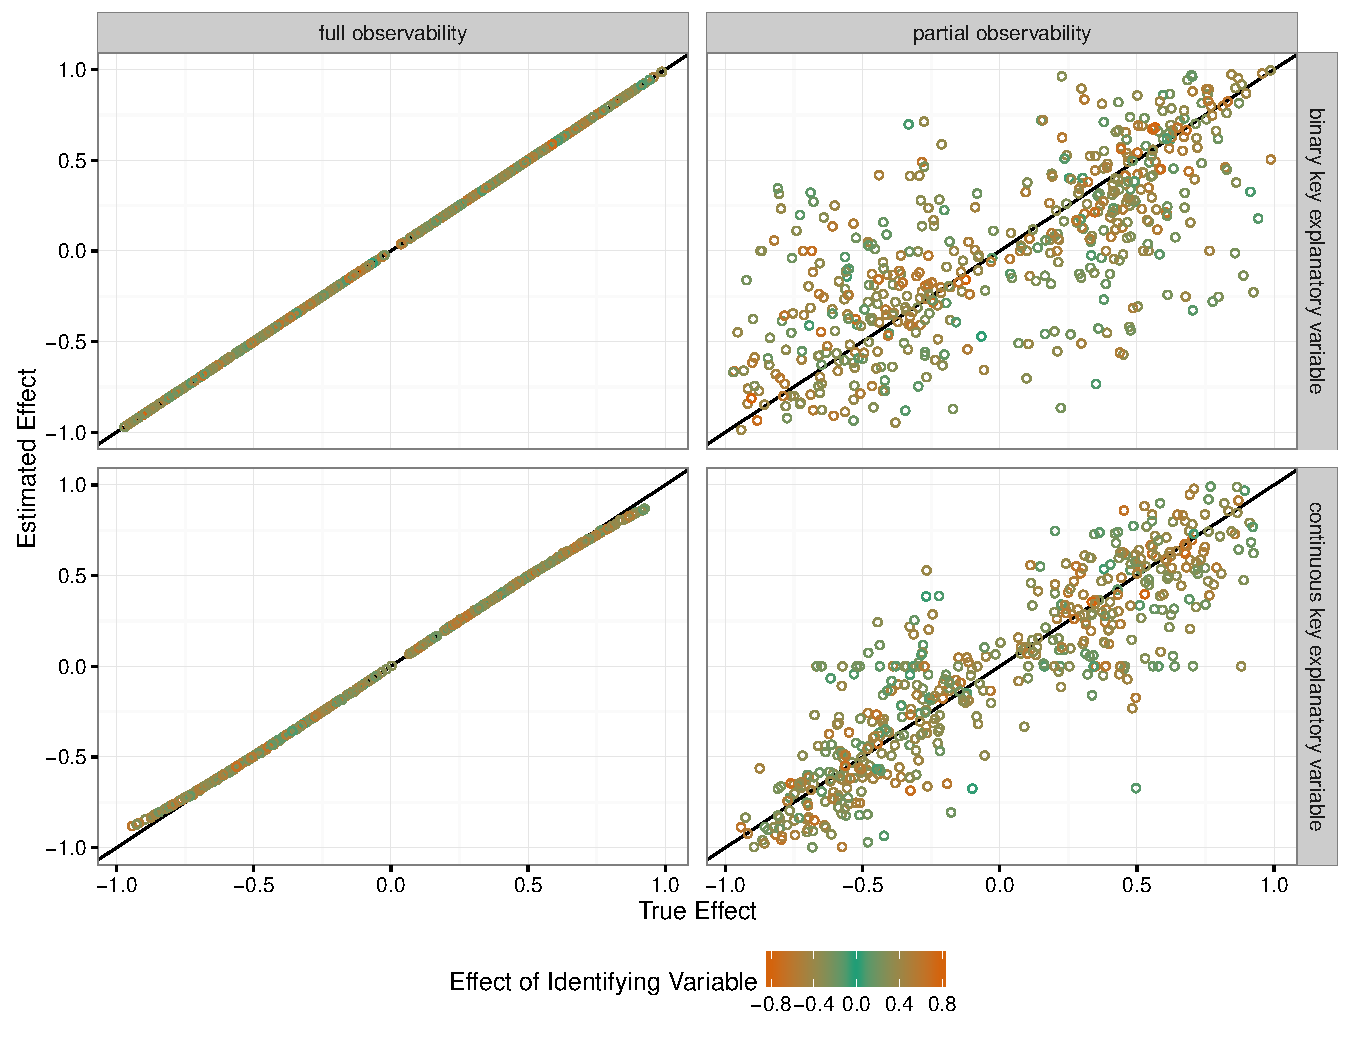
\includegraphics[scale = 0.6]{figs/mon-sims-scatter.pdf}
\caption{These scatterplots show the large-sample estimates of the first difference as the true first difference varies. The left column shows the estimates under full observability (i.e., usual logit model) and the right column shows the estimates under partial observability. The top row shows the estimates when the key explanatory variable is binary and the bottom row shows the estimates when the key explanatory variable is continuous.}\label{fig:mon-sims}
\end{center}
\end{figure}

Though the functional form misspecification has almost no influence on the ability of the full observability logit model to estimate the effect of interest, the same misspecification causes substantial bias in the partial observability estimates. 
For a continuous $w$, the average absolute bias is about 0.19. The 95th percentile is 0.54, and the maximum bias in our sample is 1.17. 
For a binary $w$, the average absolute bias is 0.28, the 95th percentile is 0.85, and the maximum is 1.15. 
The large-sample absolute bias is larger than 0.1 in 65\% of the simulations, larger than 0.3 in 27\% of the simulations, and larger than 0.5 in 12\% of the simulations. 
To put this in perspective, many effects of interest to political scientists are smaller than 0.1. 

Sign errors are also a substantial problem for the monotonic DGP. 
When $w_1$ is binary, 19\% of the simulations produce a large-sample sign error. 
When $w_1$ is continuous, this only shrinks to about 11\%. 
In applied settings, not only do researchers need to worry about sampling error, they need to worry that the model, even with negligible sampling error, may converge to an estimate with the \textit{wrong sign}.

One might suspect that the magnitude of the bias depends on the magnitude of the effect of the identifying variable. As the magnitude of the effect of the identifying variable increases, the potential for bias does tend to decrease, but it shrinks rather slowly. The 95th percentile of the absolute bias is 1.00 when the effect of $z$ is 0.1. If $z$ has a much larger effect of 0.5, then the 95th percentile of the absolute bias only drops to 0.58.

\section*{Conclusion}

We highlight an under-appreciated but critical characteristic of partial observability models---they are quite sensitive to seemingly innocuous specification errors. 
Even small errors in the functional form can lead to a substantial bias in large samples, including sign errors.

Meng and Schmidt (1985) counseled economists early on regarding some of the costs of partial observability, arguing that standard errors are much larger when the outcome of interest is only partially observed. 
They write, ``we would not be surprised to find, in a typical application, $t$-ratios to be from two to four times as large under full observability as under partial observability'' (Meng and Schmidt 1985, p. 83). 
Yet by design, standard errors only reflect the uncertainty due to sampling error. 
Other sources of error, such as measurement error, missing data, and specification error create additional uncertainty. 
In the case of full observability, our simulations show that the functional form has a negligible impact on the large-sample estimates. 
But in the case of partial observability, uncertainty about the functional form should generate suspicion about the estimates. 
The bias introduced from specification error of the partial observability model can be quite large, is rarely negligible, and is not captured in the standard errors.

One might wonder about the possibility of model specification tests to determine the severity of the misspecification. 
We are not optimistic about this possibility. 
The motivating example shows that two models can fit the observed data exactly and still provide opposite inferences. 
In general, researchers could use a test to determine whether the partial observability model offers a good model of $\Pr(y)$. 
But researchers cannot evaluate the quality of the models of $\Pr(d_{main})$ and $\Pr(d_{nuisance})$ because these variables are unobserved.
A model might predict the observed data quite well, but offer terrible predictions for the unobserved data.
Thus, specification tests cannot resolve the issue when the researcher is interested in explaining $d_{main}$.

Recent applications are relatively sanguine about employing the partial observability model. 
For example, Przeworski and Vreeland (2002; see also Przeworski and Vreeland 2000, Vreeland 2003, and Stone 2008) are interested in how surplus in a nation's budget affects both the IMF's and the national government's decisions to enter an agreement.
They find that as a budget surplus increases, a government becomes \textit{less} likely to enter an IMF agreement, but the IMF becomes \textit{more} likely to enter an agreement.
Interestingly, and consistent with our claim, Stone (2008) uses data from a later time period and reports an \textit{opposite} effect of the budget surplus on a government's decision to participate in an agreement.
In spite of these and other optimistic applications of the partial observability model, our analysis suggests that some skepticism is in order. 
Indeed, our simulations show that relatively minor and unavoidable model specification errors can lead to a substantial large-sample bias in the estimates.

\singlespace

\section*{References}
\parskip=0.15in
\begin{hangparas}{.25in}{1}

Abowd, John M., and Henry S. Farber. 1982. ``Job Queues and the Union Status of Workers.'' \textit{Industrial and Labor Relations Review} 35:354-367.

Amir, Shmueli. 2001. ``The Effect of Health on Acute Care Supplemental Insurance Ownership: An Empirical Analysis.'' \textit{Health Economics} 10: 341-350.

Boyes, William J., Dennis L. Hoffman, and Stuart A. Low. 1989. ``An Econometric Analysis of the Bank Credit Scoring Problem." \textit{Journal of Econometrics} 40: 3-14.

Braumoeller, Bear F. 2003. ``Causal Complexity and the Study of Politics.'' \textit{Political Analysis} 11:209-233.

Braumoeller, Bear F. and Austin Carson. 2011. ``Political Irrelevance, Democracy, and the Limits of Militarized Conflict.'' \textit{Journal of Conflict Resolution} 55:292-320.

Chen, Gongmeng, Michael Firth, Daniel N. Gao, and Oliver M. Rui. 2006. ``Ownership Structure, Corporate Governance, and Fraud: Evidence from China.'' \textit{Journal of Corporate Finance} 12: 424-448.

Comola, Margherita, and Marcel Fafchamps. 2014. ``Testing Unilateral and Bilateral Link Formation.'' \textit{The Economic Journal} 124: 954-976. 

Dimara, Efthalia, and Dimitris Skuras. 2003. ``Adoption of Agricultural Innovations as a Two?Stage Partial Observability Process.'' \textit{Agricultural Economics} 28(3): 187-196.

Feinstein, Jonathan S. 1990. ``Detection Controlled Estimation.'' \textit{Journal of Law and Economics} 33:233-276.

Heywood, John S., and Madhu S. Mohanty. ``Race and Employment in the Federal Sector.'' \textit{Economics Letters} 33: 179-183.

Knight, Malcolm, and Julio A. Santaella. 1997. ``Economic Determinants of IMF Financial Arrangements.'' \textit{Journal of Development Economics} 54: 405-436.

Logan, John Allen. 1996. ``Opportunity and Choice in Socially Structured Labor Markets.'' \textit{American Journal of Sociology} 102:114-160.

Mebane Jr, Walter R., and Jasjeet S. Sekhon. 2011. ``Genetic Optimization Using Derivatives: The rgenoud Package for R.'' \textit{Journal of Statistical Software} 42: 1-26.

Meng, Chun-Lo, and Peter Schmidt. 1985. ``On the Cost of Partial Observability in the Bivariate Probit Model." \textit{International Economic Review} 26:71-85.

Mohanty, Madhu S. 2002 ``A Bivariate Probit Approach to the Determination of Employment: A Study of Teen Employment Differentials in Los Angeles County.'' \textit{Applied Economics} 34:143-156.

Nieman, Mark David. 2015. ``Statistical Analysis of Strategic Interaction with Unobserved Player Actions: Introducing a Strategic Probit with Partial Observability.'' \textit{Political Analysis} 23:429-448..

Poirier, Dale J. 1980. ``Partial Observability in Bivariate Probit Models.'' \textit{Journal of Econometrics} 12:209-217.

Przeworski, Adam, and James Raymond Vreeland. 2000. ``The Effect of IMF Programs on Economic Growth.'' \textit{Journal of Development Economics} 62:385-421.

Przeworski, Adam, and James Raymond Vreeland. 2002. ``A Statistical Model of Bilateral Cooperation.'' \textit{Political Analysis} 10:101-112.

Sekhon, Jasjeet S., and Walter R. Mebane. 1998. ``Genetic Optimization Using Derivatives.'' \textit{Political Analysis} 7(1): 187-210.

Stafford, Sarah L. 2002. ``The Effect of Punishment on Firm Compliance with Hazardous Waste Regulations.'' \textit{Journal of Environmental Economics and Management} 44: 290-308.

Stone, Randall W. 2008. ``The Scope of IMF Conditionality.'' \textit{International Organization} 62:589-620.

Tukey, John W. 1986. ``Sunset Salvo.'' \textit{The American Statistician} 40:72-76.

Vreeland, James Raymond. 2003. The IMF and Economic Development. Cambridge, UK: Cambridge University Press.

Wang, Tracy Yue. 2013. ``Corporate Securities Fraud: Insights from a New Empirical Framework.'' \textit{Journal of Law, Economics, and Organization} 29:535-568.

Xiang, Jun. 2010. ``Relevance as a Latent Variable in Dyadic Analysis of Conflict.'' \textit{Journal of Politics} 72:484-498.

\end{hangparas}

\newpage
\begin{appendix}
\begin{center}
{\LARGE \textbf{Appendix}}
\end{center}
\section{Algorithm for Wrong Link Function Simulations}\label{app:link}

\begin{enumerate}
\item Choose $n_x$ and $n_z$ independently from a Poisson distribution with mean 1.5. If both $n_x$ and $n_z$ equal zero, then set $n_z$ equal to one.
\item Choose $n_w - 1$ from a Poisson distribution with mean 0.5.
\item Assign a type (continuous or binary) to each of the $n_x + n_z + n_w$ variables with equal probability. Continuous variables take on the values 0.0, 0.2, 0.4, 0.6, 0.8, or 1.0, and binary variables take on the values 0 or 1.
\item Create a data set $WXZ$ that contains each possible combination of all of the explanatory variables.
\item Choose the preliminary coefficients $\beta^*$ and $\gamma*$ from a normal distribution. The intercept coefficients come from a normal distribution with mean 0 and standard deviation 2. The slope coefficients come from a normal distribution with mean 0 and standard deviation 1.
\item If the link function of the DGP is logit, then set $\beta$ equal to $\beta^*$ and $\gamma$ equal to $\gamma^*$. If the link function is some other function $g$, then (1) simulate a large data set from the logit DGP, (2) estimate a model with link function $g$ to that data set, and (3) set the $\beta$ and $\gamma$ equal to the estimates $\hat{\beta}$ and $\hat{\gamma}$, respectively. This step scales the coefficients so that the quantities of interest have comparable magnitude.
\item Using the parameters $\beta$ and $\gamma$, simulate 100,000,000 values of $y$ and $d_{main}$ for each combination of the explanatory variables.
\item Fit a full observability model to the outcome variable $d_{main}$. Calculate the first difference as $w_1$ moves from 0 to 1. Store this large-sample estimate.
\item Fit a partial observability model to the outcome variable $y$. Calculate the first difference as $w_1$ moves from 0 to 1. Store this large-sample estimate.
\end{enumerate}

\section{Algorithm for Monotonic Link Function Simulations}\label{app:mon}

\begin{enumerate}
\item Choose the coefficients for the non-linear, interactive equations
\begin{equation}
\Pr(d_{main}) = \beta_{cons} + \beta_w w + \beta_{w^2} w^2 \nonumber
\end{equation}
and 
\begin{equation}
\Pr(d_{nuisance}) = \gamma_{cons} + \gamma_w w + + \gamma_z z + \gamma_{w^2} w^2 + \gamma_{z^2} z^2 + \gamma_{wz} wz \text{.}\nonumber
\end{equation}
from a uniform distribution that ranges from 0 to 1.
\item check that this link function produces a monotonic relationship between the $w$ and $\Pr(d_{main})$ and between $w$ and $z$ $\Pr(d_{nuisance})$. 
\item Set $w$ as either binary or continuous. Continuous variables take on the values 0.0, 0.2, 0.4, 0.6, 0.8, or 1.0, and binary variables take on the values 0 or 1.
\item Create a data set $WZ$ that contains each possible combination of $w$ and $z$. 
\item For each row in $WZ$, simulate 100,000,000 values of $y$ and $d_{main}$.
\item Fit a full observability model to the outcome variable $d_{main}$. Calculate the first difference as $w_1$ moves from 0 to 1. Store this large-sample estimate.
\item Fit a partial observability model to the outcome variable $y$. Calculate the first difference as $w_1$ moves from 0 to 1. Store this large-sample estimate.
\end{enumerate}



\end{appendix}

\end{document}